\documentclass[11pt,letterpaper]{article}
\usepackage[utf8]{inputenc}
\usepackage[french]{babel}
\usepackage{amsmath}
\usepackage{mathtools}
\usepackage{amsfonts}
\usepackage{dsfont}
\usepackage{amssymb}
\usepackage{graphicx}
\usepackage{amsthm}
\usepackage{hyperref}
\usepackage{url}
\usepackage{float}
\usepackage{geometry}
\usepackage{enumitem}
\usepackage{framed}
\usepackage{thmtools}
\usepackage{etoolbox}
\usepackage{fancybox}
\usepackage{microtype}


% Macros personnelles.
\DeclareMathOperator*{\argmax}{arg\,max}
\DeclareMathOperator*{\argmin}{arg\,min}
\newtheorem*{ideal}{Idéal}
\newtheorem*{objectif}{Objectif}
\newtheorem{theorem}{Théorème}
\newtheorem{idee}{Idée}
\newtheorem{definition}{Définition}
\newtheorem{prop}{Proposition}
\newtheorem{cor}{Corollaire}
\newtheorem{lemme}{Lemme}

\newenvironment{myleftbar}{%
\def\FrameCommand{\hspace{0.6em}\vrule width 2pt\hspace{0.6em}}%
\MakeFramed{\advance\hsize-\width \FrameRestore}}%
{\endMakeFramed}


% Titre.
\title{A universal procedure for aggregating estimators \\ Notes}
\date{Janvier 2019}
\author{Lucas BROUX}

\begin{document}

% Title.
\maketitle


% Page of contents.
\pagebreak
\tableofcontents
\pagebreak


% Introduction.
\section{Introduction - Théorème 1}

\par Ces notes reprennent l'article \cite{goldenshluger2009universal}. 

\par Nous considérons le modèle "bruit blanc gaussien", dans lequel on observe la réalisation d'une fonction inconnue par dessus laquelle s'ajoute un bruit. Formellement, soit 
\begin{equation}
 	\quad \left|
    \begin{split}
    & d \in \mathbb{N} , \\ 
    & \mathcal{D}_0 := \left[0, 1 \right]^{d} , \\
    & W \text{ le processus de Wiener standard dans } \mathbb{R}^d , \\
    & \epsilon \in \left(0, 1 \right) \text{ correspondant au niveau de bruit}.
    \end{split}
  \right.
\end{equation}

\par On observe
\begin{equation}
\mathcal{Y}_\epsilon := \left\lbrace Y_\epsilon \left( t \right), t \in \mathcal{D}_0 \right\rbrace .
\end{equation}

\par Où
\begin{equation}
Y_\epsilon \left( dt \right) = f \left( t \right) dt + \epsilon W \left( dt \right) .
\end{equation}

\par On suppose donnés un certain nombre d'estimateurs de $f$ sous la forme $\mathcal{F}_\Theta = \left\lbrace f_\theta, \theta \in \Theta \right\rbrace$, paramétrisés par un ensemble $\Theta$.

\begin{ideal}
\par Trouver :
	\begin{equation}
		\argmin\limits_{f_\theta \in \mathcal{F}_\Theta}^{} \underbrace{\mathbb{E}_f \left[ \| f_\theta - f \|_p \right]}_{=: \mathcal{R}_p \left[f_\theta; f \right]} .
	\end{equation}
\end{ideal}

\par La difficulté du problème vient du fait que la métrique de risque dépend de la fonction inconnue $f$. En pratique, on remplace donc cet idéal par le problème suivant :

\begin{objectif}
\par Trouver un estimateur $f_{\hat{\theta}} \in \mathcal{F}_\Theta$ tel que
	\begin{equation}
		\mathcal{R}_p \left[f_{\hat{\theta}}; f \right] \leq C \inf\limits_{\theta \in \Theta} \mathcal{R}_p \left[f_\theta; f \right] + r_\epsilon .
	\label{eq:objectif}
	\end{equation}

\end{objectif}

\begin{idee}[Cours]
\par On suppose
\begin{itemize}
\item $p = 2$,
\item $f_{theta} = LSE \left( S_\theta \right)$ où $S_\theta$ est un convexe fermé de $\mathbb{L}_2 \left( \mathcal{D}_0 \right)$.
\end{itemize}
\par Dans ce cadre, on utilise
\begin{itemize}
\item La structure euclidienne de $\mathbb{L}_2 \left( \mathcal{D}_0 \right)$ pour maitriser le risque.
\item Une inégalité de concentration gaussienne pour maitriser le processus isonormal.
\end{itemize}
\par Sous hypothèses supplémentaires, on peut montrer une inégalité de type \eqref{eq:objectif}.
\end{idee}

\begin{idee}[Papier]
\par On ne fait pas d'hypothèses sur les $f_\theta$. Pour simplifier on suppose $\mathcal{F}_\Theta = \mathcal{F}_{\underbrace{\left\lbrace 1, \cdots, N \right\rbrace}_{=: I_N}}$; et $p \in \left[ 1, + \infty \right]$.
\end{idee}

\par Explorons désormais ce cadre. 

\subsection{Le théorème général}

\par Question : comment quantifier la distance de $f$ à $f_i$ ? L'idée est de déléguer la question à un ensemble de fonctions tests. On considère donc une famille de fonctions à ajuster ultérieurement

\begin{equation}
\Psi := \left\lbrace \psi : \mathcal{D}_0 \to \mathbb{R} \right\rbrace
\end{equation}

\par Et on teste la pertinence de $f_i$ en calculant

\begin{equation}
	\begin{split}
		\Delta_i \left( \psi \right) & := \int_{\mathcal{D}_0}^{} \psi \left( t \right) Y_\epsilon \left( dt \right) - \int_{\mathcal{D}_0}^{} \psi \left( t \right) f_i \left( t \right) dt \\
		&= \int_{\mathcal{D}_0}^{} \psi \left( t \right) \left[ f \left( t \right) - f_i \left( t \right) \right] dt + \epsilon \underbrace{\int_{\mathcal{D}_0}^{} \psi \left( t \right) W \left( dt \right)}_{=: \underbrace{Z \left( \psi \right)}_{Gaussien}} .
	\end{split}
\end{equation}

\par Ainsi, mis à part le terme de bruit $Z \left( \psi \right)$, contrôler $\Delta_i \left( \psi \right)$ uniformément en $\psi$, c'est contrôler la "distance" de $f$ à $f_i$. Autrement dit, sauf en cas de grandes déviations de $Z$, $\Delta$ permet de bien contrôler la "distance" entre $f$ et $f_i$.

\par Rigoureusement, on fixe $\delta > 0$ et on considère

\begin{equation}
\chi := \chi \left( \delta, \Psi \right) := \min \left\lbrace x > 0, \mathbb{P} \left[ \underbrace{ \sup\limits_{\psi \in \Psi} \frac{\left| Z \left( \psi \right) \right|}{\left\| \psi \right\|_2} \geq x }_{=: A_x^c} \right] \leq \delta \right\rbrace .
\end{equation}

\par Ainsi sur l'événement $A_\chi$, de probabilité $\geq 1 - \delta$, on a
\begin{equation}
\sup\limits_{\psi \in \Psi} \frac{\left| Z \left( \psi \right) \right|}{\left\| \psi \right\|_2} \leq \chi 
\end{equation}

\par Donc sur $A_\chi$, 
\begin{equation}
	\begin{split}
		\left| \Delta_i \left( \psi \right) \right| \leq \left| \int_{\mathcal{D}_0}^{} \psi \left( t \right) \left[ f \left( t \right) - f_i \left( t \right) \right] dt \right| + \epsilon \chi \left\| \psi \right\|_2 .
	\end{split}
\end{equation}

\par Et donc sur $A_\chi$, 
\begin{equation}
	\begin{split}
		\left| \Delta_i \left( \psi \right) \right| - \epsilon \chi \left\| \psi \right\|_2 & \leq \int_{\mathcal{D}_0}^{} \left| \psi \left( t \right) \left[ f \left( t \right) - f_i \left( t \right) \right| \right] dt \\
		& \overbrace{\leq}^{Holder} \left\| \psi \right\|_q \left\| f - f_i \right\|_p .
	\end{split}
\end{equation}

\par Conclusion : sauf sur un événement de probabilité $\leq \delta$, 
\begin{equation}
	\begin{split}
		\underbrace{\sup\limits_{\psi \in \Psi} \left( \frac{\left| \Delta_i \left( \psi \right) \right| - \epsilon \chi \left\| \psi \right\|_2}{\left\| \psi \right\|_q} \right)}_{=: \hat{M}_i, \text{ connu par observation}} \leq \underbrace{\left\| f - f_i \right\|_p}_{\text{inconnu, quantité voulue}} .
	\end{split}
\end{equation}

\par Cela nous dicte notre procédure :
\begin{itemize}
\item On choisit $\hat{i} := \argmin\limits_{i \in I_N} \hat{M}_i$.
\item On retourne $\hat{f} := f_{\hat{i}}$.
\end{itemize}

\par Evaluons la qualité de notre procédure. Pour cela, on écrit
\begin{equation}
	\begin{split}
		\left\| f - \hat{f} \right\|_p = \left\| f - \hat{f} \right\|_p \mathds{1}_{A_\chi} + \left\| f - \hat{f} \right\|_p \mathds{1}_{A_\chi^c} .
	\end{split}
\end{equation}

\par Donc 
\begin{equation}
	\begin{split}
		\mathcal{R}_p \left[\hat{f}; f \right] & = \mathbb{E}_f \left[ \left\| f - \hat{f} \right\|_p \mathds{1}_{A_\chi} \right] + \mathbb{E}_f \left[ \left\| f - \hat{f} \right\|_p \mathds{1}_{A_\chi^c} \right] \\
		& \leq \mathbb{E}_f \left[ \left\| f - \hat{f} \right\|_p \mathds{1}_{A_\chi} \right] + \max_{i \in I_N} \left( \left\| f \right\|_p + \left\| f_i \right\|_p \right) \delta .
	\end{split}
\end{equation}

\par Ainsi, on veut contrôler $\left\| f - \hat{f} \right\|_p$ en fonction de 
\begin{equation}
	\begin{split}
		\min\limits_{i \in I_N} \left\| f - f_i \right\|_p =: \left\| f - f_{i^*} \right\|_p .
	\end{split}
\end{equation}

\par Or sous $A_\chi$,
\begin{equation}
	\begin{split}
		\left\| f - \hat{f} \right\|_p \leq \left\| f - f_{i^*} \right\|_p + \left\| f_{i^*} - \hat{f} \right\|_p .
	\end{split}
\end{equation}

\par Reste donc à contrôler $\left\| f_{i^*} - \hat{f} \right\|_p$. C'est le moment de demander des comptes à nos fonctions tests !

\begin{definition}
\par On dit que $\Psi$ est $\left( \gamma, p \right)$-good si pour tout $i \neq j \in I_N$, il existe $\psi_{i, j} \in \Psi$ tel que 
\begin{equation}
	\begin{split}
		\left| \left\| f_i - f_j \right\|_p - \int_{\mathcal{D}_0}^{} \psi_{i, j} \left( t \right) \left[ f_i \left( t \right) - f_j \left( t \right) \right] dt \right| \leq \gamma .
	\end{split}
\end{equation}
\end{definition}

\par A partir de maintenant, on suppose que $\Psi$ est $\left( \gamma, p \right)$-good. Alors sous $A_\chi$,
\begin{equation}
	\begin{split}
		\left\| f_{i^*} - \hat{f} \right\|_p & = \left\| f_{i^*} - f_{\hat{i}} \right\|_p \\
		& \leq \left| \int_{\mathcal{D}_0}^{} \psi_{i^*, \hat{i}} \left( t \right) \left[ f_{i^*} \left( t \right) - f_{\hat{i}} \left( t \right) \right] dt \right| + \gamma \\
		& = \left| \Delta_{i^*} \left( \psi_{i^*, \hat{i}} \right) - \Delta_{\hat{i}} \left( \psi_{i^*, \hat{i}} \right) \right| + \gamma \\
		& \leq \left| \Delta_{i^*} \left( \psi_{i^*, \hat{i}} \right) \right| + \left| \Delta_{\hat{i}} \left( \psi_{i^*, \hat{i}} \right) \right| + \gamma \\
		&= \left( \frac{\left| \Delta_{i^*} \left( \psi_{i^*, \hat{i}} \right) \right| - \epsilon \chi \left\| \psi_{i^*, \hat{i}} \right\|_2}{\left\| \psi_{i^*, \hat{i}} \right\|_q} + \frac{\left| \Delta_{\hat{i}} \left( \psi_{i^*, \hat{i}} \right) \right| - \epsilon \chi \left\| \psi_{i^*, \hat{i}} \right\|_2}{\left\| \psi_{i^*, \hat{i}} \right\|_q} \right) \left\| \psi_{i^*, \hat{i}} \right\|_q + \gamma + 2 \epsilon \chi \left\| \psi_{i^*, \hat{i}} \right\|_2 \\
		& \leq \left( \hat{M}_{i^*} + \hat{M}_{\hat{i}} \right) \left\| \psi_{i^*, \hat{i}} \right\|_q + \gamma + 2 \epsilon \chi \left\| \psi_{i^*, \hat{i}} \right\|_2 \\
		& \leq 2 \hat{M}_{i^*} \left\| \psi_{i^*, \hat{i}} \right\|_q + \gamma + 2 \epsilon \chi \left\| \psi_{i^*, \hat{i}} \right\|_2 \\
		& \leq 2 \hat{M}_{i^*} \max\limits_{\psi \in \Psi^*} \left( \left\| \psi \right\|_q \right) + \gamma + 2 \epsilon \chi \max\limits_{\psi \in \Psi^*} \left( \left\| \psi \right\|_2 \right) \\
		& \leq 2 \left\| f - f_{i^*} \right\|_p \max\limits_{\psi \in \Psi^*} \left( \left\| \psi \right\|_q \right) + \gamma + 2 \epsilon \chi \max\limits_{\psi \in \Psi^*} \left( \left\| \psi \right\|_2 \right) .
	\end{split}
\end{equation}

\par D'où : 
\begin{theorem}

\par On fixe

\begin{equation}
 	\left|
 	\begin{split}
 	& d \in \mathbb{N} , \\ 
    & \mathcal{D}_0 := \left[0, 1 \right]^{d} , \\
    & W \text{ le processus de Wiener standard dans } \mathbb{R}^d , \\
    & \epsilon \in \left(0, 1 \right) \text{ correspondant au niveau de bruit} \\
	& \delta \in \left( 0, 1 \right) \\
	& \gamma > 0 \\
	& p \in \left[ 1, + \infty \right] . &&
    \end{split}
  \right.
\end{equation}

\par On définit
\begin{equation}
 	\left|
    \begin{split}
    & \Theta := \left\lbrace 1, \cdots N \right\rbrace =: I_N \\
    & \mathcal{F}_{I_N} = \left\lbrace f_i, i \in I_N \right\rbrace \\
    & \mathcal{G}_{I_N} := \left\lbrace f_i - f_j, i \neq j \right\rbrace \\
    & \Psi_{I_N} := \left\lbrace \psi_{i, j}, i \neq j \right\rbrace \\
    & i^{*} := \argmin\limits_{i \in I_N} \left\| f - f_i \right\|_p \\
    & \Psi_{I_N}^{*} := \left\lbrace \psi_{i^{*}, i}, i \neq i^{*} \right\rbrace .
    \end{split}
  \right.
\end{equation}

\par Notre procédure est de calculer 
\begin{equation}
 	\left|
    \begin{split}
    & \Delta_i \left( \psi \right) := \int_{\mathcal{D}_0}^{} \psi \left( t \right) Y_\epsilon \left( dt \right) -  \int_{\mathcal{D}_0}^{} \psi \left( t \right) f_i \left( t \right) dt \quad \text{pour } i \in I_N, \psi \in \Psi \\
    & \chi := \min \left\lbrace \chi > 0, \mathbb{P} \left[ \max\limits_{\psi \in \Psi_{I_N}} \frac{\left| Z \left( \psi \right) \right|}{\left\| \psi \right\|_2} \geq \chi \right] \leq \delta \right\rbrace\\
    & \hat{M}_i := \max\limits_{\psi \in \Psi_{I_N}} \left\lbrace \frac{\left| \Delta_i \left( \psi \right) \right| - \epsilon \chi \left\| \psi \right\|_2}{\left\| \psi \right\|_q} \right\rbrace \\
    & \hat{i} := \argmin\limits_{i \in I_N} \hat{M}_i \\
    & \hat{f} := f_{\hat{i}} .
    \end{split}
  \right.
\end{equation}

\par On suppose que $\Psi_{I_N}$ est $\left( \gamma, p \right)$-good par rapport à $\mathcal{G}_{I_N}$.

\par Alors :

\begin{equation}
	\begin{split}
		\mathcal{R}_p \left[ \hat{f}; f\right] \leq & \left( 2 \max\limits_{\psi \in \Psi_{I_N}^{*}} \left\| \psi \right\|_q + 1 \right) \min\limits_{i \in I_N} \left\| f - f_i \right\|_p \\
		& + 2 \chi \epsilon \max\limits_{\psi \in \Psi_{I_N}^{*}} \left\| \psi \right\|_2 + \gamma + \left( \left\| f \right\|_p + \max\limits_{i \in I_N} \left\| f_i \right\|_p \right) \delta .
	\end{split}
\end{equation}

\end{theorem}

\subsection{Cas particuliers}

\par A partir de ce résultat, plusieurs questions se posent :
\begin{itemize}
\item Quel ensemble $\Psi$ conviennent ? Pour quels $\gamma$ ?
\item Peut-on contrôler $\chi$ en fonction de $\delta$ ?
\end{itemize}

\par Dans la suite, on suppose :
\begin{itemize}
\item $\delta = \epsilon$.
\item $\max \left\lbrace \left\| f \right\|_p, \left\| f_1 \right\|_p , \cdots, \left\| f_N \right\|_p \right\rbrace := L < + \infty$.
\end{itemize}

\par Commençons par résoudre le conflit entre $\chi$ et $\delta$ : notons que par définition de $\left( \gamma, p \right)$-good, on peut choisir $\left| \Psi \right| = \frac{N \left( N - 1 \right)}{2}$. Donc 
\begin{equation}
	\begin{split}
		\mathbb{P} \left[ \sup\limits_{\psi \in \Psi} \frac{\left| Z \left( \psi \right) \right|}{\left\| \psi \right\|_2} \geq x \right] &= \mathbb{P} \left[ \bigcup\limits_{\psi \in \Psi} \left\lbrace \frac{\left| Z \left( \psi \right) \right|}{\left\| \psi \right\|_2} \geq x \right\rbrace \right] \\
		& \leq \sum\limits_{\psi \in \Psi} \mathbb{P} \left[ \underbrace{\frac{\left| Z \left( \psi \right) \right|}{\left\| \psi \right\|_2}}_{\sim \mathcal{N} \left( 0, 1 \right)} \geq x \right] \\
		& = \left| \Psi \right| e^{- \frac{x^2}{2}} \\
		& \leq N^2 e^{- \frac{x^2}{2}} .
	\end{split}
\end{equation}

\par Ainsi notre $\epsilon$-niveau correspond à 
\begin{equation}
	\begin{split}
		\chi = \sqrt{2 \log \left( \frac{N^2}{\epsilon} \right)} .
	\end{split}
\end{equation}

\par En outre, on peut expliciter plusieurs ensembles $\Psi$ intéressants :

\begin{prop}
\par Soit $p \in \left[1, +\infty \right)$, alors
\begin{equation}
	\begin{split}
		\Psi_{I_N} := \left\lbrace \psi_{i, j} := \frac{\left| \left( f_i - f_j \right) \left( . \right) \right|^{p - 1}}{\left\| f_i - f_j \right\|_p^{p - 1}} sgn \left( \left( f_i - f_j \right) \left( . \right) \right), i \neq j \right\rbrace .
	\end{split}
\end{equation}
\par est $\left( 0, p \right)$-good. Et en outre, pour tout $\psi \in \Psi$, $\left\| \psi \right\|_q = 1$.
\end{prop}


\par Dès lors, la conclusion du théorème implique
\begin{equation}
	\begin{split}
		\mathcal{R}_p \left[ \hat{f}; f\right] \leq & 3 \min\limits_{i \in I_N} \left\| f - f_i \right\|_p \\
		& + 2 \epsilon \sqrt{2 \log \left( \frac{N^2}{\epsilon} \right)} \underbrace{\max\limits_{\psi \in \Psi_{I_N}^{*}} \left\| \psi \right\|_2}_{ \leq \underbrace{\left\lbrace \substack{ 1 \quad \quad \quad \quad \quad \quad \quad \quad \text{ si } 1 \leq p \leq 2 \\ \max\limits_{i \neq i^*} \left( \frac{\left\| f_{i^*} - f_i \right\|_{2p - 2}}{\left\| f_{i^*} - f_i \right\|_{p}} \right)^{p-1} \text{ si } 2 < p < + \infty} \right.}_{=: Q_1 \left( p \right)} } +  0 + 2 L \epsilon .
	\end{split}
\end{equation}

\begin{cor}

\par On suppose les hypothèses du théorème 1, et en outre $\max \left\lbrace \left\| f \right\|_p, \left\| f_1 \right\|_p , \cdots, \left\| f_N \right\|_p \right\rbrace := L < + \infty$ et $p \in \left[1, +\infty \right)$, alors :
\begin{equation}
	\begin{split}
		\mathcal{R}_p \left[ \hat{f}; f\right] \leq & 3 \min\limits_{i \in I_N} \left\| f - f_i \right\|_p + 2 \epsilon \sqrt{2 \log \left( \frac{N^2}{\epsilon} \right)} Q_1 \left( p \right) + 2 L \epsilon .
	\end{split}
\end{equation}
\end{cor}


\subsection{Questions}

\par Quelques questions se posent :
\begin{itemize}
\item Peut-on améliorer cela lorsque $p = 2$ ? Réponse : oui, c'est facile : en exploitant la structure euclidienne sous-jacente.
\item Existe-t'il une procédure lorsque $\epsilon$ n'est pas supposé connu ? Réponse : oui, c'est facile : en modifiant légèrement notre procédure.
\item Peut-on faire de l'agrégation convexe ? Réponse : oui, ce n'est pas trop difficile, on peut expliciter une procédure similaire.
\item Le théorème est-il optimal ? Réponse : ce n'est pas évident à priori...
\end{itemize}


% Section 2. Extensions et adaptations.
\section{Inégalité minimax}

\begin{theorem}
\par On se place dans le cas $N > 3, p \in \left(2, +\infty\right]$. Alors il existe une famille de fonctions $\bar{\mathcal{F}}_{I_N} := \left\lbrace \bar{f}_i, i \in I_N \right\rbrace$ sur $\mathcal{D}_0$ telle que 
\begin{enumerate}[label=(\roman*)]
\item $\max\limits_{i \in I_N} \left\| \bar{f}_i \right\|_p \leq L $.
\item pour tous $\epsilon \leq L \left( N \log \left( N \right) \right)^{-\frac{1}{2}}$, 
\begin{equation}
	\begin{split}
		\inf\limits_{\tilde{f}: \mathcal{Y}_\epsilon \to \bar{\mathcal{F}}_{I_N} } \max\limits_{f \in \bar{\mathcal{F}}_{I_N}} \left( \mathcal{R}_p \left[ \tilde{f}; f \right] - \min\limits_{i \in I_N} \left\| f - \bar{f}_i \right\|_p \right) \geq c K_p \epsilon \sqrt{\log \left( N - 1 \right)} .
	\end{split}
\end{equation}

\end{enumerate}
\end{theorem}


\begin{proof}
\par L'idée est de considérer $B_i, i = 1, \cdots, N$ des boréliens disjoints de $\mathcal{D}_0$ de mesure de Lebesgue $h \leq \frac{1}{N}$ à ajuster; puis on pose $\bar{f}_i := L \mathds{1}_{B_i}$. Alors l'ensemble  $\bar{\mathcal{F}}_{I_N} := \left\lbrace \bar{f}_i, i \in I_N \right\rbrace$ convient. En effet, $(i)$ est vraie par construction. En outre, notons
\begin{equation}
	\begin{split}
		s := \left\| \hat{f}_i - \hat{f}_j \right\|_p = \left( 2 h \right)^{\frac{1}{p}} L .
	\end{split}
\end{equation}

\par Fixons $\tilde{f}: \mathcal{Y}_\epsilon \to \bar{\mathcal{F}}_{I_N} $. L'inégalité de Markov :
\begin{equation}
	\begin{split}
		\max\limits_{f \in \bar{\mathcal{F}}_{I_N}} \left( \mathcal{R}_p \left[ \tilde{f}; f \right] - \min\limits_{i \in I_N} \left\| f - \bar{f}_i \right\|_p \right) & = \max\limits_{i \in I_N} \left( \mathcal{R}_p \left[ \tilde{f}; f \right] \right) \\
		& \geq \frac{s}{2} \max\limits_{i \in I_N} \mathbb{P}_i \left[ \left\| \tilde{f} - \hat{f}_i \right\|_p \geq \frac{s}{2} \right] \\
		& \geq \frac{s}{2} \max\limits_{i \in I_N} \mathbb{P}_i \left[ \underbrace{ \tilde{i} \neq i }_{=: A_i} \right] .
	\end{split}
\end{equation}

\par Nous concluons avec une conséquence du lemme de Birgé :
\begin{lemme}[Birgé]
\par Soit $\left( \mathbb{P}_i \right)_{1 \leq i \leq N}$ une famille de probabilités et $\left( A_i \right)_{1 \leq i \leq N}$ une famille d'événements disjoints. Soit $K := \frac{1}{N - 1} \sum\limits_{i = 2}^{N} K \left( \mathbb{P}_i, \mathbb{P}_1 \right)$ alors
\begin{equation}
	\begin{split}
		\max\limits_{i \in I_N} \mathbb{P}_i \left( A_i \right) \geq 1 - \kappa \wedge \left( \frac{K}{\log \left( N \right)} \right) .
	\end{split}
\end{equation}

\par Où $\kappa = \frac{2 e }{2 e + 1}$ convient.
\end{lemme}

\par Ici, nous pouvons expliciter les entropies mutuelles grâce à la formule de Cameron-Martin (cf cours p. 29) : pour $i \neq j$ :
\begin{equation}
	\begin{split}
		K \left( \mathbb{P}_i, \mathbb{P}_j \right) = \frac{\left\| \bar{f}_i - \bar{f}_j \right\|_2^2}{2 \epsilon^2} = \frac{h L^2}{\epsilon^2} .
	\end{split}
\end{equation}

\par Donc 
\begin{equation}
	\begin{split}
		\max\limits_{i \in I_N} \mathbb{P}_i \left[ \underbrace{ \tilde{i} \neq i }_{=: A_i} \right] & \geq 1 - \kappa \wedge \left( \frac{h L^2}{\epsilon^2 \log \left( N \right)} \right) .
	\end{split}
\end{equation}

\par On choisit $h = \frac{\epsilon^2 \log \left( N \right)}{L^2}$ (ce qui est possible dès que $\epsilon \leq L \left( N \log
 \left( N \right) \right)^{-\frac{1}{2}}$) alors 
\begin{equation}
	\begin{split}
		\max\limits_{i \in I_N} \mathbb{P}_i \left[ \underbrace{ \tilde{i} \neq i }_{=: A_i} \right] & \geq 1 - \kappa \geq \frac{1}{7} .
	\end{split}
\end{equation}

\par Réinjectant, on obtient le résultat voulu.

\end{proof}



% Section 3. Application numérique.
\section{Application numérique}

\subsection{Cadre}

\par On observe

\begin{equation}
Y := \underbrace{\mu}_{\in \mathbb{R}^n} + \epsilon \underbrace{W}_{\sim \mathcal{N} \left( 0, \Sigma \right)} .
\end{equation}

\par La procédure mise en évidence ci-dessus s'adapte à ce cadre.

\par Pour notre expérience : 
\begin{itemize}
\item $n = 1000$.
\item $\Sigma = Id$.
\item On fixe $K$, et on calcule $\mu$ en tirant $K$ composantes du vecteur selon une loi $\mathcal{N} \left( 0, \Sigma \right)$ et les autres composantes sont nulles.
\item On tire deux variables : $Y_1 \sim \mathcal{N} \left( \mu, \epsilon_1^2 \Sigma \right)$ et $Y_2 \sim \mathcal{N} \left( \mu, \epsilon_2^2 \Sigma \right)$.
\item Nos estimateurs sont 10 estimateurs de projection et 10 estimateurs de seuil.
\end{itemize}

\subsection{Résultats}

\begin{figure}[H]
  \centering
    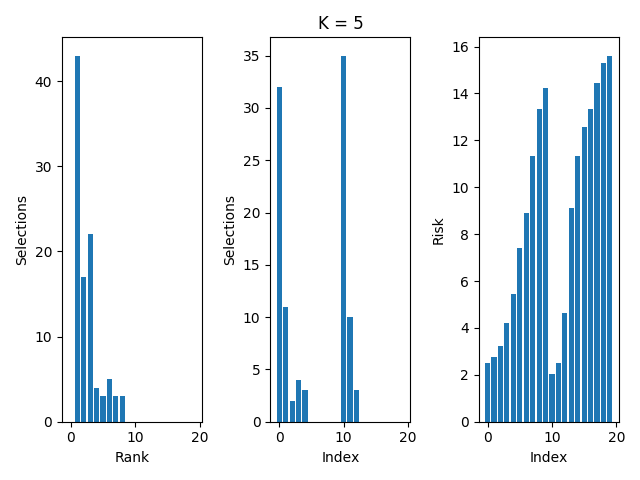
\includegraphics[width=0.7\textwidth]{images/K=5.png}
  \caption{$K = 5$.}
\end{figure}

\begin{figure}[H]
  \centering
    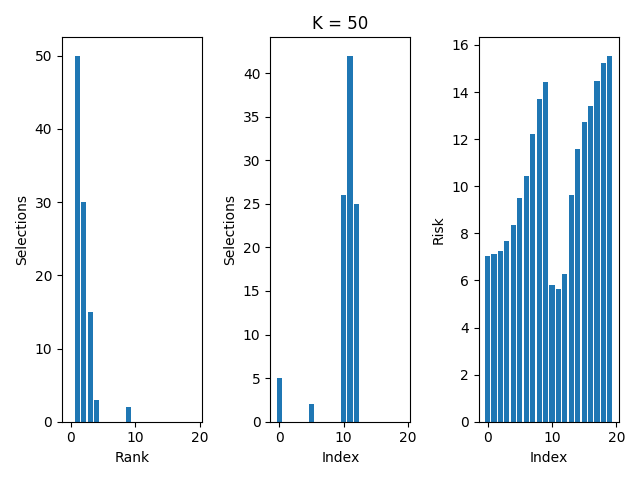
\includegraphics[width=0.7\textwidth]{images/K=50.png}
  \caption{$K = 50$.}
\end{figure}

\begin{figure}[H]
  \centering
    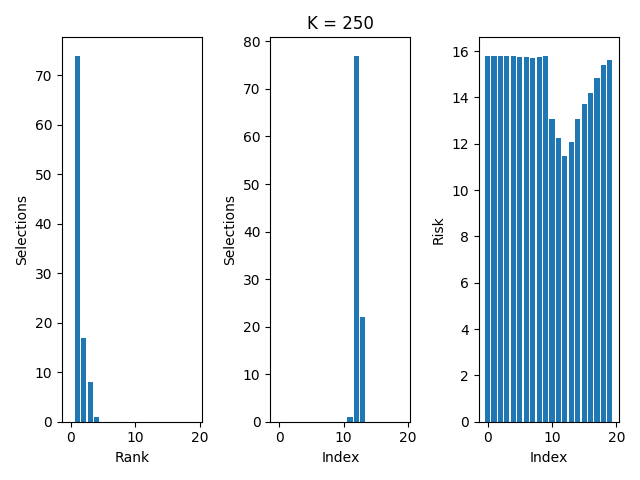
\includegraphics[width=0.7\textwidth]{images/K=250.png}
  \caption{$K = 250$.}
\end{figure}

\begin{figure}[H]
  \centering
    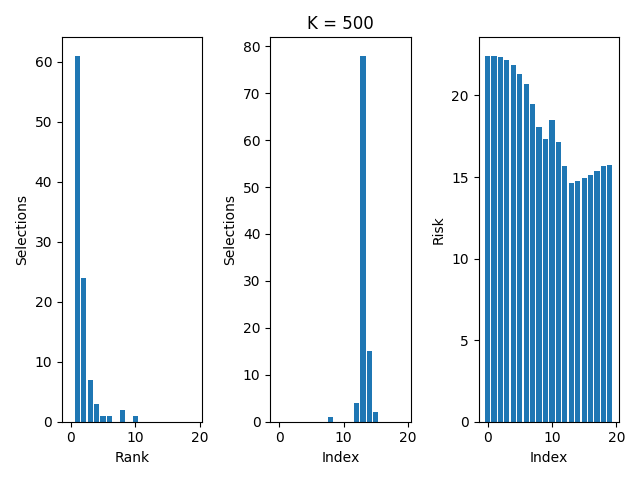
\includegraphics[width=0.7\textwidth]{images/K=500.png}
  \caption{$K = 500$.}
\end{figure}

\par On observe que l'estimateur choisi est souvent parmi les meilleurs. La procédure est relativement efficace dans tout les cas.

% Conclusion.
\section{Conclusion}

\par Dans un premier temps, nous avons introduit un estimateur naturel et universel. Nous avons établi une borne "intéressante" sur le risque de notre procédure de sélection, que nous pouvons spécifier dans divers cas particuliers. Nous avons ensuite vu que cette borne est en un sens "optimale" en établissant une borne minimax comme conséquence du lemme de Birgé. Nous avons enfin réalisé une application numérique dans le cas vectoriel, et mis en évidence la relative performance de notre critère.





% Bibliography.
\pagebreak
\nocite{*}
\bibliographystyle{plain}
\bibliography{projectbib}


\end{document}